\documentclass[english,onecolumn]{IEEEtran}
\usepackage[T1]{fontenc}
\usepackage[latin9]{luainputenc}
\usepackage[letterpaper]{geometry}
\geometry{verbose}
\usepackage{amsfonts}
\usepackage{babel}
\usepackage{ulem}

\usepackage{extarrows}
\usepackage[colorlinks]{hyperref}
\usepackage{listings}
\usepackage{xcolor}
\usepackage[ruled,linesnumbered]{algorithm2e}

\usepackage{amsmath,graphicx}
\usepackage{subfigure} 
\usepackage{cite}
\usepackage{amsthm,amssymb,amsfonts}
\usepackage{textcomp}
\usepackage{bm,pifont}
\usepackage{booktabs}
\usepackage{listings}
\usepackage{xparse}
\usepackage{xcolor}
\definecolor{salmon}{rgb}{1, 0.5020, 0.4471}

\NewDocumentCommand{\codeword}{v}{
\texttt{\textcolor{blue}{#1}}
}

\lstdefinestyle{mystyle}{
    backgroundcolor=\color{backcolour},   
    commentstyle=\color{codegreen},
    keywordstyle=\color{magenta},
    numberstyle=\tiny\color{codegray},
    stringstyle=\color{codepurple},
    basicstyle=\ttfamily\footnotesize,
    breakatwhitespace=false,         
    breaklines=true,                 
    captionpos=b,                    
    keepspaces=true,                 
    numbers=left,                    
    numbersep=5pt,                  
    showspaces=false,                
    showstringspaces=false,
    showtabs=false,                  
    tabsize=2
}

\lstset{style=mystyle}

\providecommand{\U}[1]{\protect\rule{.1in}{.1in}}
\topmargin            -18.0mm
\textheight           226.0mm
\oddsidemargin      -4.0mm
\textwidth            166.0mm
\def\baselinestretch{1.5}


\newtheorem{theorem}{Theorem}[section]
\newtheorem{lemma}[theorem]{Lemma}

\newcommand{\Rbb}{\mathbb{R}}
\newcommand{\Pb}{\mathbf{P}}
\newcommand{\Ib}{\mathbf{I}}
\newcommand{\vb}{\mathbf{v}}
\newcommand{\Ucal}{\mathcal{U}}
\newcommand{\Wcal}{\mathcal{W}}
\newcommand{\Vcal}{\mathcal{V}}
\newcommand{\Rcal}{\mathcal{R}}
\newcommand{\Ncal}{\mathcal{N}}
\newcommand{\bigO}{\mathcal{O}}
\newcommand{\bigS}{\mathcal{S}}
\newcommand{\bA}{{\bf A}}
\newcommand{\bQ}{{\bf Q}}
\newcommand{\bR}{{\bf R}}
\newcommand{\bH}{{\bf H}}
\newcommand{\bU}{{\bf U}}
\newcommand{\bT}{{\bf T}}
\newcommand{\bI}{{\bf I}}
\newcommand{\bq}{{\bf q}}
\newcommand{\bz}{{\bf z}}
\newcommand{\bL}{{\bf L}}
\newcommand{\bx}{{\bf x}}
\newcommand{\bv}{{\bf v}}
\newcommand{\bG}{{\bf G}}
\def\A{\mathbf{A}}
\def\v{\mathbf{v}}

\begin{document}

\begin{center}
	\textbf{\LARGE{SI231 - Matrix Computations, Fall 2020-21}}\\
	{\Large Homework Set \#4}\\
	\texttt{Prof. Yue Qiu and Prof. Ziping Zhao}\\
	\texttt{\textbf{Name:}}   	\texttt{ LiuChang }  		\hspace{1bp}
	\texttt{\textbf{Major:}}  	\texttt{ Master in IE } 	\\
	\texttt{\textbf{Student No.:}} 	\texttt{ 2020232161}     \hspace{1bp}
	\texttt{\textbf{E-mail:}} 	\texttt{ liuchang3@shanghaitech.edu.cn}
\par\end{center}

\noindent
\rule{\linewidth}{0.4pt}
{\bf {\large Acknowledgements:}}
\begin{enumerate}
    \item Deadline: \textcolor{red}{\textbf{2020-11-20 23:59:00}}
    \item Submit your homework at \textbf{Gradescope}.
    Homework \#4 contains two parts, the theoretical part the and the programming part.
    \item About the the theoretical part:
    \begin{enumerate}
            \item[(a)] Submit your homework in \textbf{Homework 4} in gradescope. Make sure that you have correctly select pages for each problem. If not, you probably will get 0 point.
            \item[(b)] Your homework should be uploaded in the \textbf{PDF} format, and the naming format of the file is not specified.
            \item[(c)] No handwritten homework is accepted. You need to use \LaTeX $\,$ in principle.
            \item[(d)] Use the given template and give your solution in English. Solution in Chinese is not allowed. 
        \end{enumerate}
  \item About the programming part:
  \begin{enumerate}
      \item[(a)] Submit your codes in \textbf{Homework 4 Programming part} in gradescope. 
      \item[(b)] When handing in your homework in gradescope, package all your codes into {\sf your\_student\_id+hw4\_code.zip} and upload. In the package, you also need to include a file named {\sf README.txt/md} to clearly identify the function of each file.
     \item[(c)] Make sure that your codes can run and are consistent with your solutions.
  \end{enumerate}
  \item \textbf{Late Policy details can be found in the bulletin board of Blackboard.}
\end{enumerate}
\rule{\linewidth}{0.4pt}

\section*{Study Guide}
\noindent
This homework concerns the following topics:
\begin{itemize}
    \item Eigenvalues, eigenvectors \& eigenspaces 
    \item Algebraic multiplicity \& geometric multiplicity
    \item Eigendecomposition (Eigvenvalue decomposition) \& Eigendecomposition for Hermitian matrices
    \item Similar transformation, Schur decomposition \& 
    Diagonolization
    \item Variational characterizations of eigenvalues
	\item Power iteration \& Inverse iteration
	\item QR iteration \& Hessenberg QR iteration
	\item Givens QR \& Householder QR (from previous lectures)
\end{itemize}


\newpage 
\section{Understanding eigenvalues and Eigenvectors}

\noindent\textbf{Problem 1}. {\color{blue}(6 points + 4 points)}

\noindent
Consider the $2\times 2$ matrix \[ {\bf A} = \begin{bmatrix}
           -4 & -3 \\
            6 & 5
    \end{bmatrix}\,.    \]
\begin{enumerate}
    \item 
    Determine whether $\bA$ can be diagonalized or not. Diagonalize $\bA$ by ${\bf A} = {\bf V}{\bf \Lambda}{\bf V}^{-1}$ if the answer is "yes" or give the reason if the answer is "no".
    
    \item  Give the eigenspace of ${\bf A}$. 
    And then consider: 
    is there a matrix being similar to ${\bf A}$  but have different eigenspaces with it.
    If the answer is "yes", show an example (here you are supposed to give the specific matrix and its eigenspaces), or else explain why the answer is "no" .
\end{enumerate}

{\bf Remarks:} 
\begin{itemize}
    \item In 1), if {\bf A} can be diagonalized, you are supposed to present not only the specific diagonalized matrix but also how do you get the similarity transformation.
    If not, you should give the necessary derivations of the specific reason.
    \item In 2), if your answer is "yes", you are supposed to give the specific matrix and its eigenspaces.
    If "no", you should give the necessary derivations of the specific reason.
\end{itemize}

\noindent
\textbf{Solution.}
\begin{enumerate}
    \item
			Yes.
			According to the definition of eigenvalue, we can get $(\bf{A}-\lambda \bf{E})v=0$\\
			$\therefore |\lambda \bf{E}-\bf{A}|=
				\begin{vmatrix}
           \lambda+4 & 3 \\
            -6 & \lambda-5
		    \end{vmatrix}=0$\\
			$\therefore \lambda_1=2,\lambda_2=-1$\\
			$\therefore$ After substitution we can get: $v_1=(1,-2)^T,v_2=(1,-1)^T$\\
			$\therefore \bf{V}=(v_1,v_2)=
				\begin{bmatrix}
					1&1\\
					-2&-1\\
				\end{bmatrix}$\\
			Calculate the inverse of V.\\
			$\therefore {\bf A} = 
				\begin{bmatrix}
		           -4 & -3 \\
		            6 & 5
		    \end{bmatrix}
				={\bf V}{\bf \Lambda}{\bf V}^{-1}=
				\begin{bmatrix}
					1&1\\
					-2&-1\\
				\end{bmatrix}
				\begin{bmatrix}
					2&0\\
					0&-1\\
				\end{bmatrix}
				\begin{bmatrix}
					-1&-1\\
					2&1\\
				\end{bmatrix}$\\
    \item 
    	The eigenspace of A associated with $\lambda_1$ is $\mathcal{V}_{\lambda_1}=span\{v_1\}=span\{(1,-2)^T\}$\\
    	The eigenspace of A associated with $\lambda_2$ is $\mathcal{V}_{\lambda_2}=span\{v_2\}=span\{(1,-1)^T\}$\\
    	Yes.\\
    	Assume $\bf{B}=\bf{P}\bf{A}\bf{P}^{-1}=
    	\begin{bmatrix}
    		1&2\\
    		3&4\\
    	\end{bmatrix}
    	\begin{bmatrix}
		           -4 & -3 \\
		            6 & 5
		  \end{bmatrix}
		  \begin{bmatrix}
		           -2 &1 \\
		            1.5 & -0.5
		  \end{bmatrix}=
		  \begin{bmatrix}
    		1&2\\
    		3&4\\
    	\end{bmatrix}
    	\begin{bmatrix}
					1&1\\
					-2&-1\\
			\end{bmatrix}
			\begin{bmatrix}
					2&0\\
					0&-1\\
			\end{bmatrix}
			\begin{bmatrix}
					-1&-1\\
					2&1\\
			\end{bmatrix}
		  \begin{bmatrix}
		           -2 &1 \\
		            1.5 & -0.5
		  \end{bmatrix}=
		  \begin{bmatrix}
					-3&-1\\
					-5&-1\\
			\end{bmatrix}
			\begin{bmatrix}
					2&0\\
					0&-1\\
			\end{bmatrix}
			\begin{bmatrix}
					0.5&-0.5\\
					-2.5&1.5\\
			\end{bmatrix}$\\
			$\therefore$ The eigenspace of B associated with $\lambda_1$ is $\mathcal{V}_{\lambda_1}=span\{(-3,-5)^T\}$\\
			$\therefore$ The eigenspace of B associated with $\lambda_2$ is $\mathcal{V}_{\lambda_2}=span\{(-1,-1)^T\}$\\
\end{enumerate}


\newpage
\noindent\textbf{Problem 2}. \textcolor{blue}{(6 points $\times$ 5)}

\noindent
For a matrix ${\bf A}\in \mathbb{C}^{n\times n}$, 
$\lambda_1, \lambda_2, \ldots, \lambda_n$   are its $n$ eigenvalues 
(though some of them may be the same). 
Prove that:
\begin{enumerate}
    \item The matrix ${\bf A}$ is singular if only if 0 is an eigenvalue of it.
    \item ${\sf rank}({\bf A}) \geq$ number of nonzero eigenvalues of ${\bf A}$.
    \item If ${\bf A}$ admits an  eigendecomposition (eigenvalue decomposition), ${\sf rank}({\bf A}) =$ number of nonzero eigenvalues of ${\bf A}$.
    \item If $\A$ is Hermitian, then all of eigenvalues of $\bA$ are real.
    \item If $\A$ is Hermitian, then eigenvectors corresponding to different eigenvalues are orthogonal.
\end{enumerate}

\noindent
\textbf{Solution}
\begin{enumerate}
    \item
    	According to the definition of eigenvalue, we can get $(\bf{A}-\lambda \bf{E})v=0$\\
			$\therefore |\lambda \bf{E}-\bf{A}|=0$\\
			$\because $ 0 is an eigenvalue of A.\\
			$\therefore$ 0 is one of the solution of $|\lambda \bf{E}-\bf{A}|=0$\\
			$\therefore |\bf{A}|=0$ which means A is singular.
    \item
    	Assume the number of nonzero eigenvalues of A is k.\\
    	$\therefore$ 0 is n-k repeated root.\\
    	$\therefore Av=0$ has most n-k roots.\\
    	$\therefore dim\mathcal{N}(A)\leq n-k$\\
    	$\because Av=\lambda v$\\
    	$\therefore rank(A)=rank(A^T)=dim\mathcal{R}(A^T)=dim\mathcal{N}(A)^{\perp}=n-dim\mathcal{N}(A)\geq k$\\
    	Proved.
    \item
    	$\because $ A can be eigendecomposited.\\
    	$\therefore rank(A)=rank(V\Lambda V^{-1})\leq min\{rank(V),rank(\Lambda)\}$\\
    	$\because rank(V)=n$\\
    	$\therefore rank(A)\leq rank(\Lambda)=$number of nonzero eigenvalues of ${\bf A}$\\
    	As I have proved above, $rank(A)=$number of nonzero eigenvalues of ${\bf A}.$
    \item 
    	According to the definition of Hermitian, $A=A^H$\\
			$\because Av=\lambda v$\\
			$\therefore v^HA^H=\bar{\lambda}v^H$\\
			$\therefore v^HA=\bar{\lambda}v^H $\\
			$\therefore v^HAv=\bar{\lambda}v^Hv$\\
			$\therefore v^H\lambda v=\bar{\lambda}v^Hv$\\
			$\because v^Hv$ is numeral.\\
			$\therefore \lambda=\bar{\lambda}$\\
			$\therefore$ All of eigenvalues of $\bA$ are real.			
    \item 
    	$\because Av_1=\lambda_1v_1$\\
    	$\therefore v_1^HA^H=\bar{\lambda_1}v_1^H$\\
    	$\therefore v_1^HAv_2=\bar{\lambda_1}v_1^Hv_2$\\
    	$\therefore v_1^H\lambda_2v_2=\bar{\lambda_1}v_1^Hv_2$\\
			$\therefore v_1^H\lambda_2v_2=\lambda_1v_1^Hv_2$\\
    	According to the question, $\lambda_1\neq\lambda_2$\\
    	$\therefore v_1^Hv_2=0$\\
    	$\therefore$ Eigenvectors corresponding to any two different eigenvalues are orthogonal.\\
\end{enumerate}

\clearpage
\section{Understanding The Eigenvalues of Real Symmetric Matrices}
\noindent\textbf{Problem 3}. \textcolor{blue}{(12 points)}
\noindent 
Let $\bA\in \Rbb^{n\times n}$ be a symmetric matrix, $\bigS_k$ denote a subspace of $\Rbb^n$ of dimension $k$, and $\lambda_1\geq \lambda_2\geq...\geq \lambda_n$ represent the eigenvalues of $\bA$. 
For any $k\in\{1,2,3,...,n\}$, prove that \[\lambda_k=\min\limits_{\bigS_{n-k+1}\subseteq \Rbb^n}\max\limits_{\bx\in\bigS_{n-k+1},||\bx||_2=1} \bx^T\bA\bx.\]

\noindent
\textbf{Solution.}\\
Assume $N=\bigS_{n-k+1}=span\{u_1,...u_{n-k+1}\}$ and $u_1,...u_{n-k+1}$ are orthogonal\\
Assume $ \bx\in N$\\
$\therefore x=\sum_{i=1}^{n-k+1} \alpha_{i} u_{i}$\\
$\because ||x||_2=1$\\
$\therefore \sum_{i=1}^{n-k+1} \alpha_{i}^2=1$\\
$\therefore \bx^T\bA\bx=\sum_{i=1}^{n-k+1}\alpha_{i}^2 u_{i}^T\bA u_i=\sum_{i=1}^{n-k+1}\alpha_{i}^2\lambda_i$(according to the defination of eigenvalue)\\
$\because \lambda_i  in  \sum_{i=1}^{n-k+1}\alpha_{i}^2\lambda_i$ is randomly picked in $\lambda_1...\lambda_n$\\
$\therefore \max\limits_{\bx\in\bigS_{n-k+1},||\bx||_2=1}\sum_{i=1}^{k+1}\alpha_{i}^2\lambda_i$ means the max$\alpha_{i}^2$ corresponding to the max$\lambda_i$\\
$\because \lambda_1\geq \lambda_2\geq...\geq \lambda_n$\\
$\therefore \min\limits_{\bigS_{n-k+1}\subseteq \Rbb^n}\max\limits_{\bx\in\bigS_{n-k+1},||\bx||_2=1}\sum_{i=1}^{k+1}\alpha_{i}^2\lambda_i$ means $\{u_1,...u_{n-k+1}\}$ corresponding to the min$\{\lambda_1,...\lambda_{n-k+1}\}$ \\
$\therefore \{u_1,...u_{n-k+1}\}$ corresponding to the $\{\lambda_{k},...\lambda_{n}\}$\\
$\therefore \alpha_k^2=1$\\
$\therefore$max$\lambda_i=\lambda_k$\\
$\therefore \min\limits_{\bigS_{n-k+1}\subseteq \Rbb^n}\max\limits_{\bx\in\bigS_{n-k+1},||\bx||_2=1} \bx^T\bA\bx=\min\limits_{\bigS_{n-k+1}\subseteq \Rbb^n}\max\limits_{\bx\in\bigS_{n-k+1},||\bx||_2=1}\sum_{i=1}^{k+1}\alpha_{i}^2\lambda_i=\lambda_k$\\
Proved.\\








\newpage
\noindent\textbf{Problem 4}. \textcolor{blue}{(5 points+8 points+10 points)}
\noindent To assist the understanding of this problem, we first provide some \textbf{basic concepts of graph theory:}
 
\ding{172} A \textit{simple graph} $G$ is a pair $(V,E)$, such that
\begin{itemize}
	\item 
	$V$ is the set of vertices;
	
	\item 
	$E$ is the set of edges and every edge is denoted by an \textit{unordered} pair of its two \textit{distinct} vertices.
\end{itemize}


\ding{173} If $i,j$ are two distinct vertices and $(i,j)$ is an edge, we then say that $i$ and $j$ are \textit{adjacent}. A graph is called $d$-regular graph if every vertex in the graph is adjacent to $d$ vertices, where $d$ is a positive integer.

\ding{174} Given two graphs $G_1=(V_1,E_1)$ and $G_2=(V_2,E_2)$, if $V_1\subset V_2$ and $E_1\subset E_2$, we call $G_1$ the \textit{subgraph} of $G_2$. 
Furthermore,  we call $G_1$ the \textit{connected component} of $G_2$ 
if 
\begin{itemize}
    \item 
	any vertex in $G_1$ is only connected to vertices in $G_1$.
	\item 
	any two vertices in $G_1$ are connected either directly or via some other vertices in $G_1$;
\end{itemize}
\vspace{3mm}
\noindent 
Suppose $G=(V,E)$ is a simple graph with $n$ vertices indexed by $1,2,...,n$ respectively. 
The adjacency matrix of $G$ is a matrix $\bA\in \Rbb^{n\times n}$ given by

\begin{equation}
\bA_{i,j}=\left\{
\begin{aligned}
1 &, \text{ if vertex } i \text{ and vertex } j \text{ are adjacent;}\\
0 &, \text{ otherwise.}
\end{aligned}
\right.
\end{equation}
Besides, if $G$ is a $d$-regular graph, its \textit{normalized Laplacian matrix} $\bL$ is defined as $\bL\triangleq \bI-\frac{1}{d}\bA$, where $\bI$ is the identity matrix. 
Let $\lambda_1\geq \lambda_2\geq...\geq \lambda_n$ denote the eigenvalues of $\bL$. 
Please prove the following propositions:
\begin{enumerate}
    \item For any vector $\bx \in \Rbb^n$, it follows that 
	\begin{equation}
	\label{C1+}
		\bx^T\bL\bx=\frac{1}{d}\sum_{(i,j)\in E}(\bx_i-\bx_j)^2,
	\end{equation} 
	where $i,j$ represent two distinct vertices and $(i,j)\in E$ represents an edge between $i$ and $j$ in the graph $G$.
	\item $\lambda_n=0$ and $\lambda_1\leq 2$.
	\item {\color{blue}(\textbf{Bonus Problem)}} the graph $G$ has at least $(n-k+1)$ connected components if and only if $\lambda_k=0$. 
\end{enumerate}



\noindent\textbf{Hint:} 
The matrix $\bL$ is real and symmetric. 
	You can directly utilize Courant-Fischer Theorem without proof. Particularly, you may need to utilize the min-max form of the Courant-Fischer Theorem for the Bonus Problem.


\noindent
\textbf{Solution}
\begin{enumerate}
	\item
		$\bx^T\bL\bx=
		\bx^T(I-\frac{1}{d}A)\bx=
		x^Tx-\frac{1}{d}x^TAx=
		\sum_{i=1}^nx_i^2-\frac{1}{d}x^TAx=
		\sum_{i=1}^nx_i^2-\frac{1}{d}\sum_{i=1}^nx^Ta_ix_i=
		\sum_{i=1}^nx_i^2-\frac{1}{d}\sum_{i=1}^n\sum_{j=1}^nx_ja_{ij}x_i$\\
		$\because $ The edge in the E is exclusive.\\
		$\therefore \bx^T\bL\bx=
		\sum_{i=1}^nx_i^2-\frac{1}{d}\sum_{(i,j)\in E}2 x_j x_i=
		\frac{1}{d}(\sum_{i=1}^n d x_i^2-\sum_{(i,j)\in E}2 x_j x_i)$\\
		$\because $ G is a d-regular graph, which means every column of A has d ones.\\
		$\therefore \bx^T\bL\bx=
		\frac{1}{d}(\sum_{i=1}^n\sum_{j=1}^n a_{ij} x_i^2-\sum_{(i,j)\in E}2 x_j x_i)=
		\frac{1}{d}(\sum_{(i,j)\in E} 2 x_i^2-\sum_{(i,j)\in E}2 x_j x_i)=
		\frac{1}{d}(\sum_{(i,j)\in E}  x_i^2-2 x_j x_i +x_j^2)=
		\frac{1}{d}(\sum_{(i,j)\in E}  ({x_i-x_j)}^2)$\\
		Proved.
	\item
		$\because \bx^T\bL\bx=\frac{1}{d}\sum_{(i,j)\in E}(\bx_i-\bx_j)^2 \geq 0$\\
		$\therefore $ L is semi-definite.\\
		$\therefore \lambda_1,...,\lambda_n \geq 0$\\
		Assume $x_k=k(1,1,1,...,1)^T$\\
		$\therefore \bx_k^T\bL\bx_k=0$\\
		$\therefore \bL\bx_k=0$\\
		$\therefore \lambda_k\bx_k=0$\\
		$\because \lambda_1\geq \lambda_2\geq...\geq \lambda_n$\\
		$\therefore \lambda_n=0$\\
		Proved.
	\item
\end{enumerate}

%%%%%%%%%%%%%%%%%%%%%%%%%%%%%%%%%%%%%%%%%%%%%%%%%%%%%%%%%%%%%%%%%%%%%%
%%%%%%%%%%%%%%%%%%%%%%%%%%%%%%%%%%%%%%%%%%%%%%%%%%%%%%%%%%%%%%%%%%%%%%

\newpage

\section{Eigenvalue Computations}
\subsection{Power Iteration} 
\noindent
\textbf{Problem 5.}
\textcolor{blue}{(20 points)}

Consider the $2\times 2$ matrix $\bA$
\[
\bA = \begin{bmatrix}
	0 & \alpha \\
	\beta & 0
\end{bmatrix}\,,\quad \text{ with }\alpha,\beta > 0\,.
\]
\begin{enumerate}
    \item Find the eigenvalues and eigenvectors of $\bA$ by hand. \textcolor{blue}{(5 points)}
    \item Program \textbf{the power iteration} (See Algorithm \ref{alg:power_iter}) and \textbf{the inverse iteration} (See Algroithm \ref{alg:inverse_iter}) respectively and report the output of two algorithms for $\bA$ (you can determine $\alpha,\beta$ by yourself), do the two algorithms converge or not? Report what you have found (you can use plots to support your analysis). \textcolor{blue}{(10 points: programming takes 5 points and the analysis takes 5 points)}
    After a few iterations, the sequence given by the power iteration fails to converge, explain why. \textcolor{blue}{(5 points)}
    (\textbf{After-class exercise:} If you want, you can study the case for other randomly generated matrices.)
\end{enumerate}
\textbf{Remarks:}
Programming languages are not restricted. In \codeword{Matlab}, you are free to use \codeword{[v,D] = eig(A)} to generate the eigenvalues and eigenvectors of $\bA$ as a reference to study  the convergence.

\begin{algorithm}[htbp]
	\label{alg:power_iter}
	\SetKwInOut{Input}{Input}\SetKwInOut{Output}{Output}
	\caption{Power iteration}
	\SetAlgoLined
	\Input{$\bA \in \mathbb{C}^{n\times n}$}
	\textbf{Initilization:} random choose $\bq^{(0)}$.\\
	\For{$k= 1,\ldots, $}{
		$\bz^{(k)} = \bA \bq^{(k-1)}$ \\
		$\bq^{(k)} = \bz^{(k)}/ \|\bz^{(k)}\|_2$\\
		$\lambda^{(k)} = (\bq^{(k)})^H\bA \bq^{(k)}$
	}
	\Output{$\lambda^{(k)}$}
\end{algorithm}

\begin{algorithm}[htbp]
	\label{alg:inverse_iter}
	\SetKwInOut{Input}{Input}\SetKwInOut{Output}{Output}
	\caption{Inverse iteration}
	\SetAlgoLined
	\Input{$\bA \in \mathbb{C}^{n\times n}$, $\mu$}
	\textbf{Initilization:} random choose $\bq^{(0)}$.\\
	\For{$k= 1,\ldots, $}{
		$\bz^{(k)} = (\bA - \mu \bI)^{-1} \bq^{(k-1)}$ \\
		$\bq^{(k)} = \bz^{(k)}/ \|\bz^{(k)}\|_2$\\
		$\lambda^{(k)} = (\bq^{(k)})^H\bA \bq^{(k)}$
	}
	\Output{$\lambda^{(k)}$}
\end{algorithm}
\noindent
\textbf{Solution}
\begin{enumerate}
    \item
    	$\because (A-\lambda E)v=0$\\
    	$\therefore \begin{vmatrix}
    		-\lambda&\alpha\\
    		\beta&-\lambda\\
    		\end{vmatrix}=0$\\
    	$\therefore \lambda_1=\sqrt{\alpha\beta},\lambda_2=-\sqrt{\alpha\beta}$\\
    	After substitution we can get:$v_1=(1,-\sqrt{\frac{\beta}{\alpha}})^T,v_2=(1,\sqrt{\frac{\beta}{\alpha}})^T$
    \item
    	The answer of power iteration:
    	\begin{figure}[ht]
    		\centering
		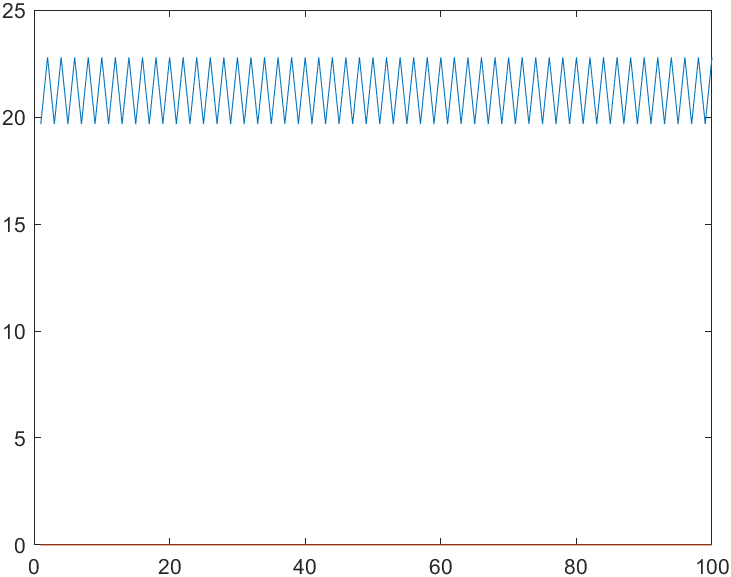
\includegraphics[scale=0.7]{power.png}
	\end{figure}\\
	The answer of inverse iteration:
    	\begin{figure}[ht]
    		\centering
		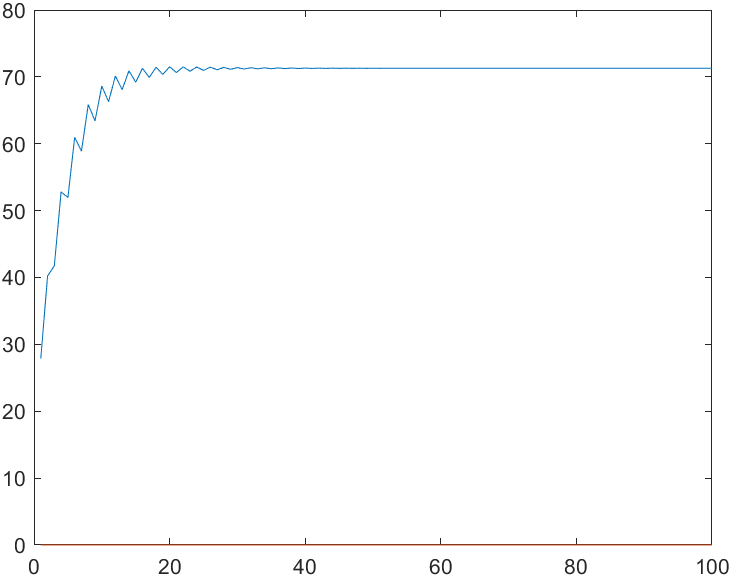
\includegraphics[scale=0.7]{inverse.png}
	\end{figure}\\
	I found the result of Power Iteration can't converge.\\
	$\because $ The assumptions of Power Iteration includes $|\lambda_1|>|\lambda_2|$\\
	$\because \left\|\mathbf{r}_{k}\right\|_{2} \leq \sum_{i=2}^{n}\left|\frac{\alpha_{i}}{\alpha_{1}}\right|\left|\frac{\lambda_{i}}{\lambda_{1}}\right|^{k}\left\|\mathbf{v}_{i}\right\|_{2} \leq\left|\frac{\lambda_{2}}{\lambda_{1}}\right|^{k} \sum_{i=2}^{n}\left|\frac{\alpha_{i}}{\alpha_{1}}\right|$ won't change if $|\lambda_1|=|\lambda_2|$\\
    	$\therefore $ Power Iteration can't work for this A.\\
\end{enumerate}


\newpage 
\subsection{QR itertiaon and Hessenberg QR iteration}
\noindent
\textbf{Recap.}
For $\bA \in \mathbb{C}^{n\times n}$,
consider the QR iteration (See Algorithm \ref{alg:qr_iter}) for finding all the eigenvalues and eigenvectors of $\bA$. 
\begin{algorithm}[htbp]
	\label{alg:qr_iter}
	\SetKwInOut{Input}{Input}\SetKwInOut{Output}{Output}
	\caption{QR iteration}
	\SetAlgoLined
	\Input{$\bA \in \mathbb{C}^{n\times n}$}
	\textbf{Initilization:} $\bA^{(0)} = \bA$.\\
	\For{$k= 1,\ldots, $}{
		$\bQ^{(k)}\bR^{(k)} = \bA^{(k-1)}$ \textcolor{blue}{\texttt{ \% Perform QR for $\bA^{(k-1)}$}}\\
		$\bA^{(k)} = \bR^{(k)}\bQ^{(k)}$
	}
	\Output{$\bA^{(k)}$}
\end{algorithm}
In each iteration, $\bA^{(k)}$ is similar to $\bA$ in that 
\begin{align*}
 	\bA^{(k)}
 	&  = \bR^{(k)}\bQ^{(k)} = (\bQ^{(k)})^H \bQ^{(k)}\bR^{(k)}\bQ^{(k)} = (\bQ^{(k)})^H \bA^{(k-1)}\bQ^{(k)}= \cdots \\
 	& = (\bQ^{(1)}\bQ^{(2)} \cdots \bQ^{(k)})^H \bA (\bQ^{(1)}\bQ^{(2)} \cdots \bQ^{(k)})  \Rightarrow \bA^{(k)} \text{ is similar to } \bA\,.
\end{align*}
Suppose the Schur decomposition of $\bA$ is $\bA = \bU \bT \bU^H$, then under some mild assumptions, $\bA^{(k)}$ converges to $\bT$.
Therefore, we can compute all the eigenvalues of $\bA$ by taking the diagonal elements of $\bA^{(k)}$ for sufficiently large $k$.
However, each iteration requires $\bigO(n^3)$ flops to compute QR factorization which is computationally expensive.
\begin{algorithm}[htbp]
	\label{alg:hessen_qr_iter}
	\SetKwInOut{Input}{Input}\SetKwInOut{Output}{Output}
	\caption{Hessenberg QR iteration}
	\SetAlgoLined
	\Input{$\bA \in \mathbb{C}^{n\times n}$}
	\textbf{Initilization:} $\bH = \bQ^H \bA \bQ\,,\bA^{(0)} = \bH$.  \textcolor{blue}{\texttt{ \% Hessenberg reduction for $\bA$}}\\
	\For{$k= 1,\ldots, $}{
		$\bQ^{(k)}\bR^{(k)} = \bA^{(k-1)}$ \textcolor{blue}{\texttt{ \% Perform QR for $\bA^{(k-1)}$ using Givens QR}}\\
		$\bA^{(k)} = \bR^{(k)}\bQ^{(k)}$ \textcolor{blue}{\texttt{ \% Matrix computation}}
	}
	\Output{$\bA^{(k)}$}
\end{algorithm}
One possible solution is: first perform similarity transform $\bA$ to an upper Hessenberg form (Step 1 in Algorithm \ref{alg:hessen_qr_iter}), then perform QR iteration (Algorithm \ref{alg:qr_iter}) over new $\bA^{(0)} = \bH$.
By using Givens rotations, the QR step only takes $\bigO(n^2)$ flops. 

\clearpage
\textbf{Problem 6.}
\textcolor{blue}{(15 points +10 points)}

\noindent
\begin{enumerate}
    \item Complete the Algorithm \ref{alg:hessen_qr_step} (corresponding to the step 3-4 of Algrorithm \ref{alg:hessen_qr_iter} ) first \textcolor{blue}{(7 points)}, then
show \textbf{the detailed derivation} of the computational complexity of in Algorithm \ref{alg:hessen_qr_step} ($\bigO(n^2)$). \textcolor{blue}{(8 points)}
(Derivation is for the computaional complexity of the algorithm.)

To be more specific, we can present the process of performing QR for $\bA^{(k)}$ using Givens rotations as:
\begin{enumerate}
\item[(a)] First, overwrite $\bA^{(k)}$ with upper-triangular $\bR^{(k)}$
\[
\bA^{(k)} = (\bG_{m}^H \bG_{m-1}^H \cdots \bG_{1}^H) \bA^{(k)} = \bR^{(k)}\,,
\]
where $\bG_{1},\ldots,\bG_{m}$ is a sequence of Givens rotations for some $m$ (In your algorithm, you need to clearly specify what $\bG_i$ is), and $\bR^{(k)}=\bG_1 \cdots \bG_{m}$.
\item[(b)] Perform matrix multiplication such that $\bA^{(k)}$ is of Hessenberg form,
\[
\bA^{(k)} = \bR^{(k)}\bQ^{(k)} = \bA^{(k)}\bG_1 \cdots \bG_{m}\,.
\]
\end{enumerate}
\item 
\textcolor{blue}{\textbf{(Bouns Problem})}
\textbf{Implicit QR iteration}

Another way to implement step 3-4 in Algorithm \ref{alg:hessen_qr_iter} is through \textit{implicit QR iteration}.
The idea is as follows, for $\bA^{(0)}\in \mathbb{R}^{n\times n}$ which is of Hessenberg form,
\begin{enumerate}
    \item[(a)] First, compute a Givens rotation $\bG_1$ such that $(\bG_1^{H}\bA^{(0)})_{2,1} =0$ and update $\bA^{(1)}  = \bG_1^{H} \bA^{(0)} \bG_1$. However, the entry $\bA^{(1)}_{3,1}$ may be nonzero (known as "bulge").
    \item[(b)] Compute another Givens rotation $\bG_2$ such that $(\bG_2\bA^{(1)})_{3,1} =0 $ (i.e., nulling out the "bulge") and update $\bA^{(2)}  = \bG_2^{H} \bA^{(1)} \bG_2$ which is analogous with step (a). Note that the entry $\bA^{(2)}_{4,2}$ will now be nonzero.
    \item[(c)] Then, we try to find $\bG_3$ such that $(\bG_3\bA^{(2)})_{4,2}=0$.
    The procedure of iterating nulling out the "bulges" to reset in a upper Hessenberg form is known as "bulge chasing".
\end{enumerate}
This algorithm \textit{implicitly} computed QR factorization at the cost of $\bigO(n^2)$, and this is why the algorithm is called the \textit{Implicit QR iteration}.
Consider a $4\times 4$ Hessenberg matrix
\[
\bA^{(0)} = \begin{bmatrix}
       1 & 2 & 3 & 4\\
       2 & 3 & 1 & 2\\
       0 & 1 & 3 & 2 \\
       0 & 0 & 2& 1
\end{bmatrix}\,.
\]
Carry out the implicit QR iteration (show the detailed derivation) (To simplify the computation, you can use \codeword{Matlab} to do the matrix multiplications. Specifically, explicitly show $\bG_i$, $\bG_i^H\bA^{(i-1)}$ and $\bA^{(i)}$ for each step but when computing the matrix multiplication such as $\bG_i^H\bA^{(i-1)}$, $\bG_i^H\bA^{(i-1)}\bG_i$, you are free to use \codeword{Matlab}. But be careful with the precision issue during the process of computing.), and observe where does the so-called "bulge" appears. \textcolor{blue}{(5 points: including the detailed derivation of the implicit QR iteration and pointing out the "bulge")}
Based on your observations, explain why the implicit QR iteration is indeed equivalent to the Algorithm \ref{alg:hessen_qr_step}. \textcolor{blue}{(5 points)}
\end{enumerate}




\begin{algorithm}[htbp]
	\label{alg:hessen_qr_step}
	\SetKwInOut{Input}{Input}\SetKwInOut{Output}{Output}
	\caption{Step 3-4 in Hessenberg QR iteration}
	\SetAlgoLined
	\Input{$\bA^{(k-1)} \in \mathbb{C}^{n\times n}$ which is of upper Hessenberg form \textcolor{blue}{\texttt{ \% corresponding to $\bA^{(k-1)}$ in step 3 of Algorithm \ref{alg:hessen_qr_iter}}}} 
	\textcolor{blue}{\texttt{ \% Perform QR for $\bA^{(k)}$ using Givens roations}}\\
		$g_{m,m}=g_{n,n}=\frac{A_{m,m}}{\sqrt{A_{m,m}^2+A_{n,m}^2}}$\\
		$g_{m,n}=-g_{n,m}=\frac{A_{n,m}}{\sqrt{A_{m,m}^2+A_{n,m}^2}}$\\
		$\mathbf{R}^{(k)}=(\begin{bmatrix}
			I&0&0\\
			0&g_{m,m}&g_{m,n}\\
			0&g_{n,m}&g_{n,n}\\
		\end{bmatrix}_{n\times n} \bG_{m-1}^H \cdots \bG_{1}^H)\mathbf{A}^{(k-1)}$\\
		
		
	\textcolor{blue}{\texttt{ \% Matrix computation}}\\
	$\mathbf{A}^{(k)}=\mathbf{R}^{(k)} (\bG_{1} \bG_{2} \cdots \bG_{m})$\\
	\Output{$\bA^{(k)}$ \textcolor{blue}{\texttt{ \% corresponding to $\bA^{(k)}$ in step 4 of Algorithm \ref{alg:hessen_qr_iter}}}}
\end{algorithm}


\noindent
\textbf{Solution}
\begin{enumerate}
    \item
    	The complexity of calculating one G : 4.\\
    	The complexity of calculating (n-1) G : 4(n-1).\\
    	The complexity of calculating $(\bG_{m}^H \bG_{m-1}^H \cdots \bG_{1}^H) \bA^{(k)}$ : 3(n+2)(n-1).\\
    	The complexity of calculating $\mathbf{R}^{(k)} (\bG_{1} \bG_{2} \cdots \bG_{m})$ : 3(n+2)(n-1).\\
    	The whole complexity=6(n+2)(n-1)+4n=$O(n^2)$.
    	
    \item
\end{enumerate}

\end{document}